\documentclass{article}
\usepackage{graphicx} % Required for inserting images
\usepackage{pgffor}
\usepackage{listings}
\usepackage{xcolor}

\lstdefinestyle{python}{
  language=Python,
  basicstyle=\ttfamily,
  numbers=left,
  numberstyle=\tiny,
  keywordstyle=\color{blue},
  commentstyle=\color{green!60!black},
  stringstyle=\color{red},
  frame=single,
  breaklines=true,
  showstringspaces=false,
}

\title{Parameter Estimation and Inverse Theory\\ Assignment 2}
\author{Parth Gupte}
\date{13th September 2023}

\begin{document}

\maketitle
\section{Experimental Procedure:}
In this experiment I created a travel time tomography simulation, using low resolution images from popular videogame minecraft.\\
\subsection{Forward Modelling Operator:}
I considered the pixel values of black and white images as the travel time.\\
Then I passed rays of light through these cells, in the end getting total travel time as the sum of each pixel crossed by the ray.\\
To build the forward modelling operator I did the following:
\begin{itemize}
    \item Convert the image into greyscale.
    \item Pass parallel rays from the left, bottom and 2 diagonals of the image and record the travel time of each ray.
    \item Create a zero array with rows for each ray and columns for each pixel.
    \item Assign value 1 to cells in each row that were in the path of the ray. This gives us forward modelling operator F.
    \item In the corresponding position place the sum of the pixel values of the rays path as the data value. This gives the d matrix.  
    \item 5\% noise gaussian was added in d for noise computations. 
\end{itemize}

\subsection{Tikonov Estimation:}
Performed Tikonov estimation using the following formula:
\begin{displaymath}
    m_{est} = (F^TF+kI)^{-1}F^Td 
\end{displaymath}
\begin{displaymath}
    F^{\dagger} = (F^TF+kI)^{-1}F^T
\end{displaymath}
Where $k > 0$\\
I used $k = 0.1$ for all calulations.

\section{Results:}
\subsection{Outputs:}
Listed below are the original images, recovered images, model resolution matrix, and the data resolution matix
for many images calculated using above scheme. The following images are taken from the popular videogame minecraft.\\
All images are less than 32x32 pixels in size
\subsubsection{Without Noise:}
Inverted images without noise:
\clearpage
\begin{itemize}
    \item alban-modified
\begin{figure}[h]
    \centering
    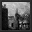
\includegraphics[width=0.6\textwidth]{images/greyscale/alban-modified.png}
    \caption{Original Image}
\end{figure}
\begin{figure}[h]
    \centering
    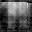
\includegraphics[width=0.6\textwidth]{images/outputs/alban-modified.png}
    \caption{Recovered Image}
\end{figure}
\begin{figure}[h]
    \centering
    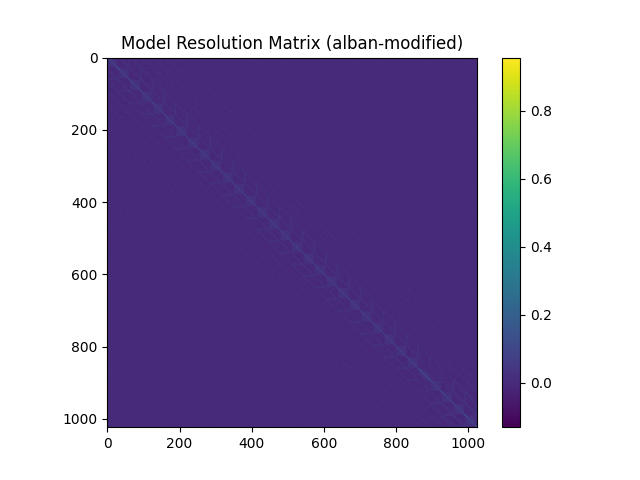
\includegraphics[width=1\textwidth]{images/outputs/modelres/alban-modified.png}
    \caption{Model Resolution Matrix}
\end{figure}
\begin{figure}[h]
    \centering
    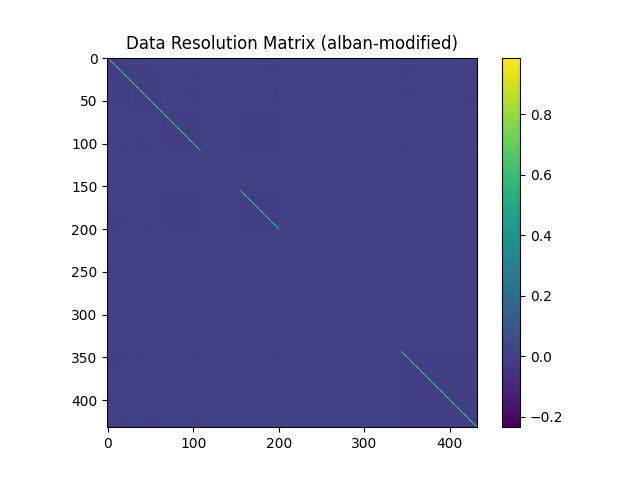
\includegraphics[width=1\textwidth]{images/outputs/datares/alban-modified.png}
    \caption{Data Resolution Matrix}
\end{figure}
\clearpage


    \item aztec-modified
\begin{figure}[h]
    \centering
    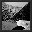
\includegraphics[width=0.6\textwidth]{images/greyscale/aztec-modified.png}
    \caption{Original Image}
\end{figure}
\begin{figure}[h]
    \centering
    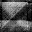
\includegraphics[width=0.6\textwidth]{images/outputs/aztec-modified.png}
    \caption{Recovered Image}
\end{figure}
\begin{figure}[h]
    \centering
    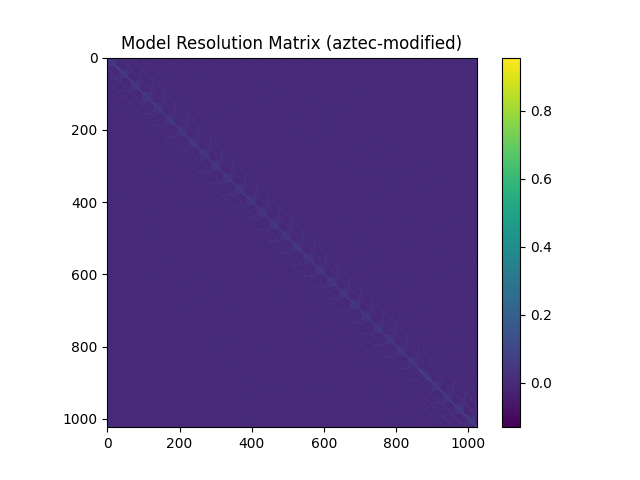
\includegraphics[width=1\textwidth]{images/outputs/modelres/aztec-modified.png}
    \caption{Model Resolution Matrix}
\end{figure}
\begin{figure}[h]
    \centering
    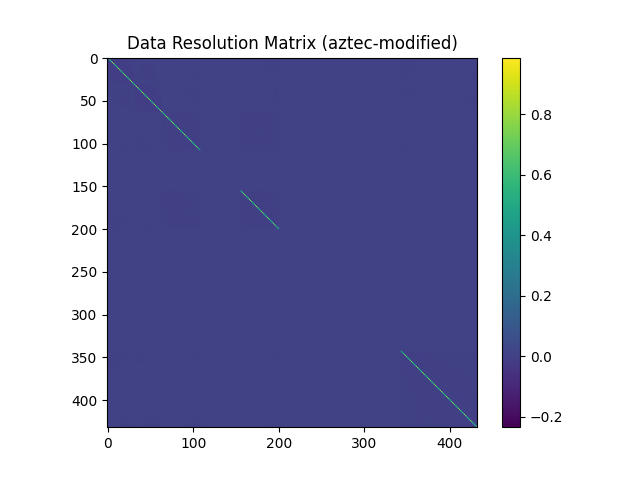
\includegraphics[width=1\textwidth]{images/outputs/datares/aztec-modified.png}
    \caption{Data Resolution Matrix}
\end{figure}
\clearpage


    \item bee\_nest\_front\_honey-modified
\begin{figure}[h]
    \centering
    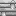
\includegraphics[width=0.6\textwidth]{images/greyscale/bee_nest_front_honey-modified.png}
    \caption{Original Image}
\end{figure}
\begin{figure}[h]
    \centering
    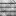
\includegraphics[width=0.6\textwidth]{images/outputs/bee_nest_front_honey-modified.png}
    \caption{Recovered Image}
\end{figure}
\begin{figure}[h]
    \centering
    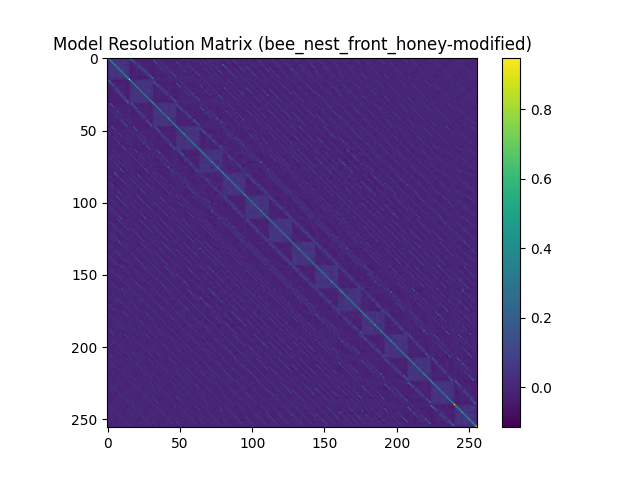
\includegraphics[width=1\textwidth]{images/outputs/modelres/bee_nest_front_honey-modified.png}
    \caption{Model Resolution Matrix}
\end{figure}
\begin{figure}[h]
    \centering
    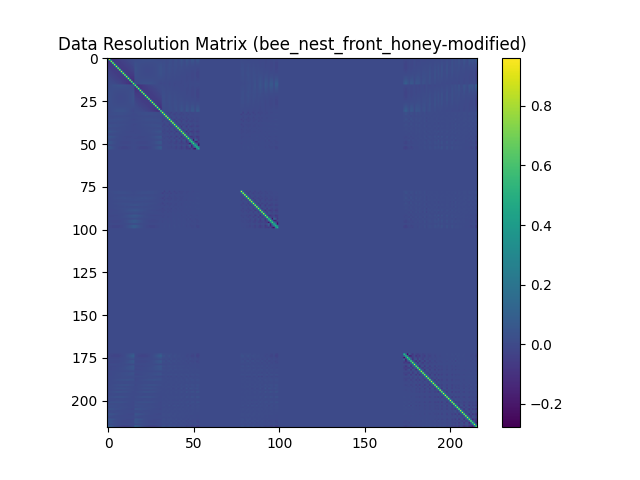
\includegraphics[width=1\textwidth]{images/outputs/datares/bee_nest_front_honey-modified.png}
    \caption{Data Resolution Matrix}
\end{figure}
\clearpage


    \item carved\_pumpkin-modified
\begin{figure}[h]
    \centering
    
\includegraphics[width=0.6\textwidth]{images/greyscale/carved_pumpkin-modified.png}
    \caption{Original Image}
\end{figure}
\begin{figure}[h]
    \centering
    
\includegraphics[width=0.6\textwidth]{images/outputs/carved_pumpkin-modified.png}
    \caption{Recovered Image}
\end{figure}
\begin{figure}[h]
    \centering
    
\includegraphics[width=1\textwidth]{images/outputs/modelres/carved_pumpkin-modified.png}
    \caption{Model Resolution Matrix}
\end{figure}
\begin{figure}[h]
    \centering
    
\includegraphics[width=1\textwidth]{images/outputs/datares/carved_pumpkin-modified.png}
    \caption{Data Resolution Matrix}
\end{figure}
\clearpage


    \item cow
\begin{figure}[h]
    \centering
    
\includegraphics[width=0.6\textwidth]{images/greyscale/cow.png}
    \caption{Original Image}
\end{figure}
\begin{figure}[h]
    \centering
    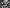
\includegraphics[width=0.6\textwidth]{images/outputs/cow.png}
    \caption{Recovered Image}
\end{figure}
\begin{figure}[h]
    \centering
    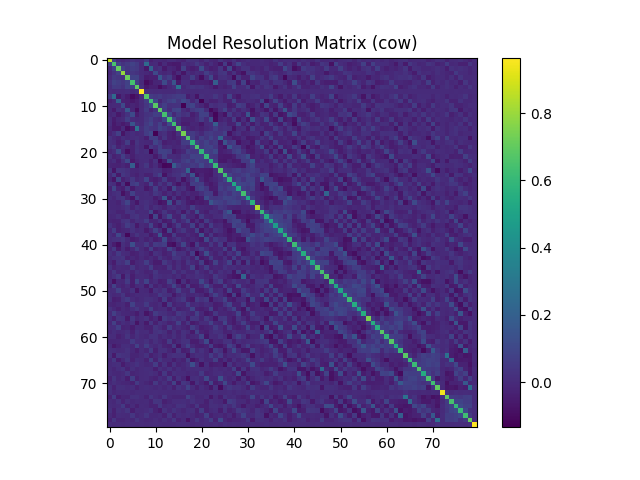
\includegraphics[width=1\textwidth]{images/outputs/modelres/cow.png}
    \caption{Model Resolution Matrix}
\end{figure}
\begin{figure}[h]
    \centering
    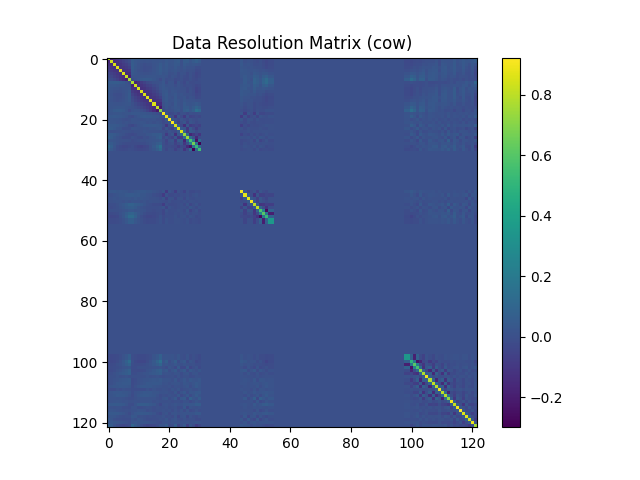
\includegraphics[width=1\textwidth]{images/outputs/datares/cow.png}
    \caption{Data Resolution Matrix}
\end{figure}
\clearpage


    \item creeper
\begin{figure}[h]
    \centering
    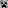
\includegraphics[width=0.6\textwidth]{images/greyscale/creeper.png}
    \caption{Original Image}
\end{figure}
\begin{figure}[h]
    \centering
    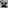
\includegraphics[width=0.6\textwidth]{images/outputs/creeper.png}
    \caption{Recovered Image}
\end{figure}
\begin{figure}[h]
    \centering
    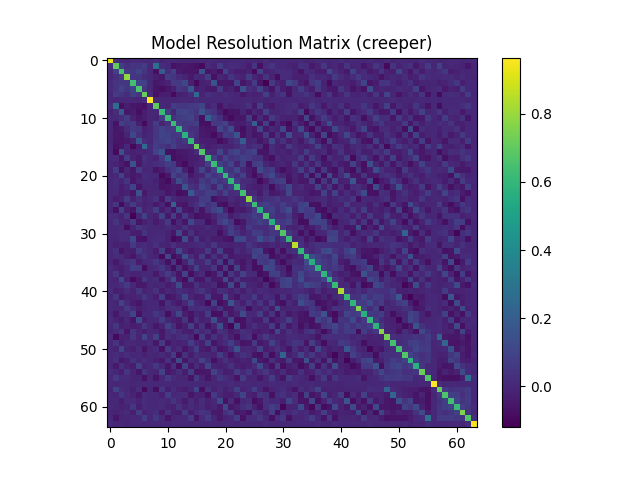
\includegraphics[width=1\textwidth]{images/outputs/modelres/creeper.png}
    \caption{Model Resolution Matrix}
\end{figure}
\begin{figure}[h]
    \centering
    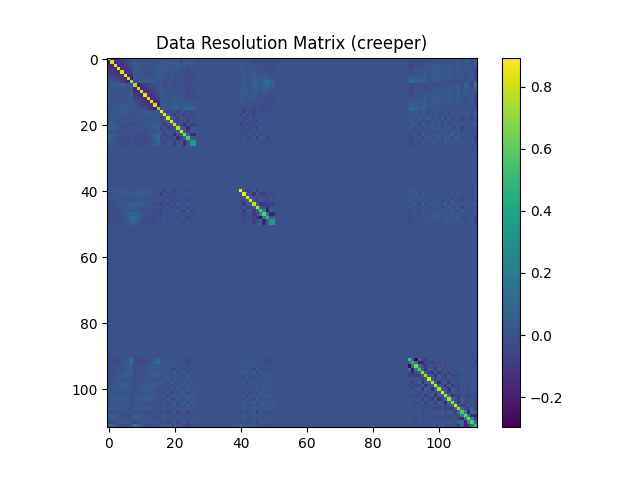
\includegraphics[width=1\textwidth]{images/outputs/datares/creeper.png}
    \caption{Data Resolution Matrix}
\end{figure}
\clearpage


    \item sheep
\begin{figure}[h]
    \centering
    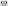
\includegraphics[width=0.6\textwidth]{images/greyscale/sheep.png}
    \caption{Original Image}
\end{figure}
\begin{figure}[h]
    \centering
    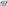
\includegraphics[width=0.6\textwidth]{images/outputs/sheep.png}
    \caption{Recovered Image}
\end{figure}
\begin{figure}[h]
    \centering
    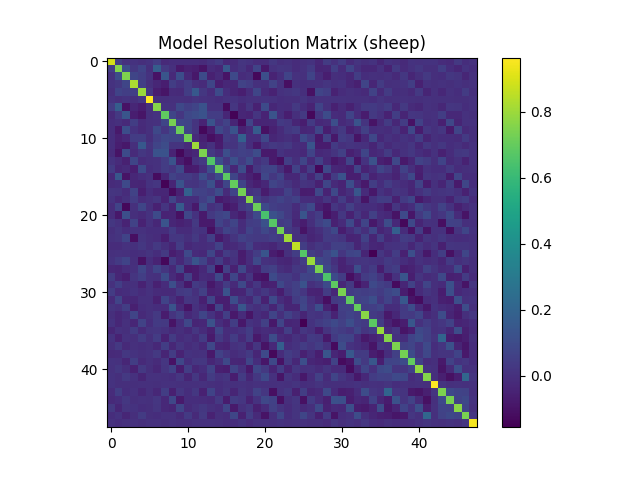
\includegraphics[width=1\textwidth]{images/outputs/modelres/sheep.png}
    \caption{Model Resolution Matrix}
\end{figure}
\begin{figure}[h]
    \centering
    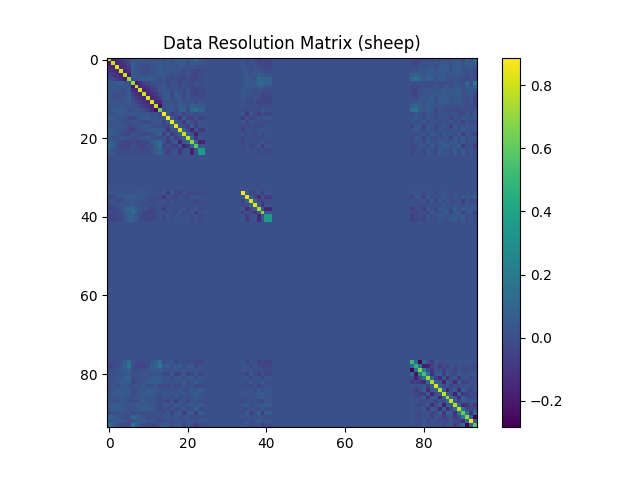
\includegraphics[width=1\textwidth]{images/outputs/datares/sheep.png}
    \caption{Data Resolution Matrix}
\end{figure}
\clearpage


    \item skeleton
\begin{figure}[h]
    \centering
    
\includegraphics[width=0.6\textwidth]{images/greyscale/skeleton.png}
    \caption{Original Image}
\end{figure}
\begin{figure}[h]
    \centering
    
\includegraphics[width=0.6\textwidth]{images/outputs/skeleton.png}
    \caption{Recovered Image}
\end{figure}
\begin{figure}[h]
    \centering
    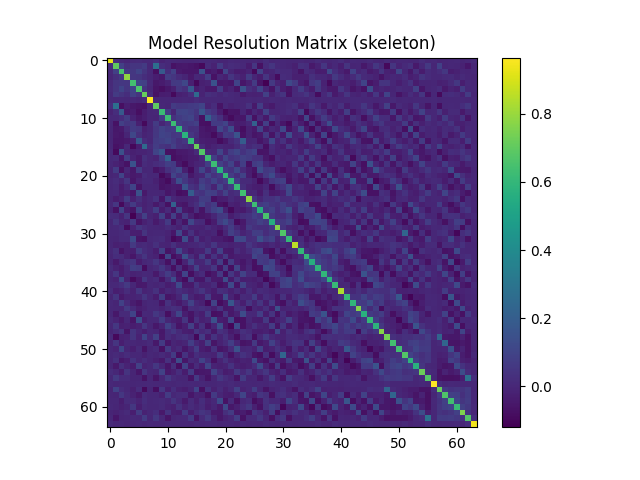
\includegraphics[width=1\textwidth]{images/outputs/modelres/skeleton.png}
    \caption{Model Resolution Matrix}
\end{figure}
\begin{figure}[h]
    \centering
    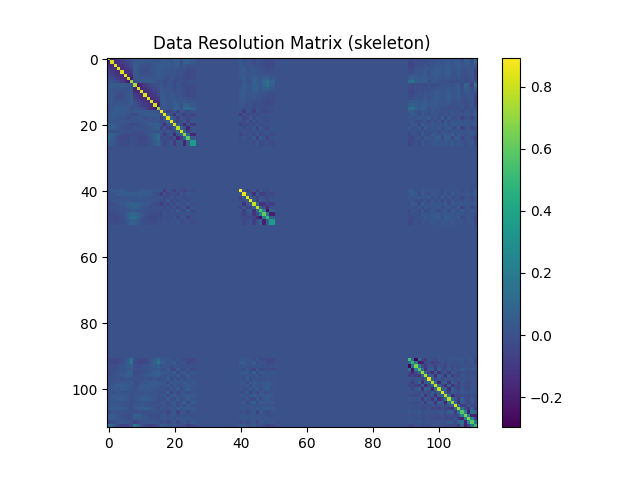
\includegraphics[width=1\textwidth]{images/outputs/datares/skeleton.png}
    \caption{Data Resolution Matrix}
\end{figure}
\clearpage


    \item steve
\begin{figure}[h]
    \centering
    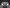
\includegraphics[width=0.6\textwidth]{images/greyscale/steve.png}
    \caption{Original Image}
\end{figure}
\begin{figure}[h]
    \centering
    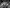
\includegraphics[width=0.6\textwidth]{images/outputs/steve.png}
    \caption{Recovered Image}
\end{figure}
\begin{figure}[h]
    \centering
    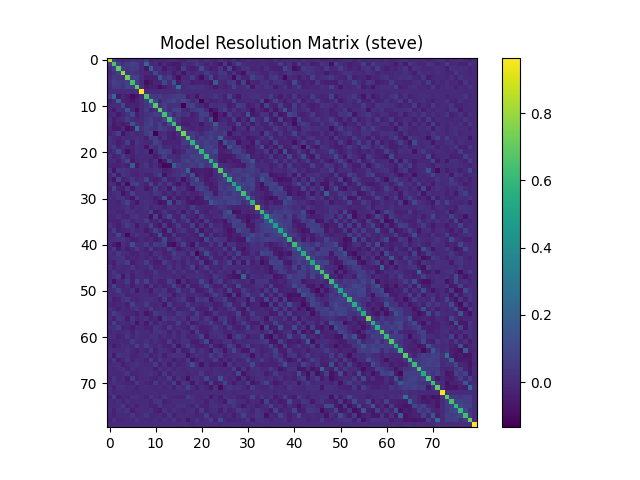
\includegraphics[width=1\textwidth]{images/outputs/modelres/steve.png}
    \caption{Model Resolution Matrix}
\end{figure}
\begin{figure}[h]
    \centering
    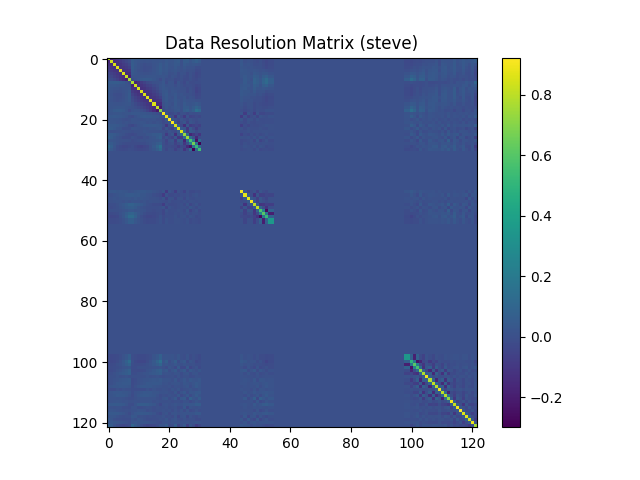
\includegraphics[width=1\textwidth]{images/outputs/datares/steve.png}
    \caption{Data Resolution Matrix}
\end{figure}
\clearpage


    \item zombie
\begin{figure}[h]
    \centering
    
\includegraphics[width=0.6\textwidth]{images/greyscale/zombie.png}
    \caption{Original Image}
\end{figure}
\begin{figure}[h]
    \centering
    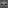
\includegraphics[width=0.6\textwidth]{images/outputs/zombie.png}
    \caption{Recovered Image}
\end{figure}
\begin{figure}[h]
    \centering
    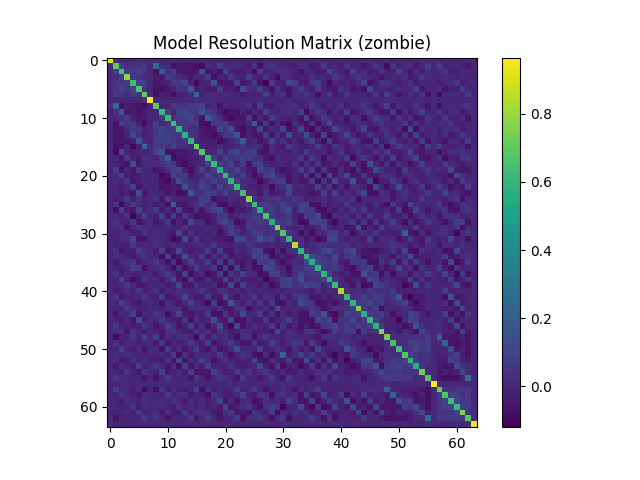
\includegraphics[width=1\textwidth]{images/outputs/modelres/zombie.png}
    \caption{Model Resolution Matrix}
\end{figure}
\begin{figure}[h]
    \centering
    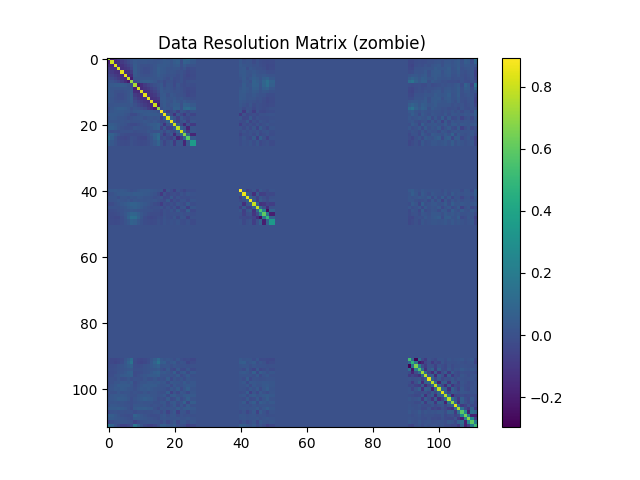
\includegraphics[width=1\textwidth]{images/outputs/datares/zombie.png}
    \caption{Data Resolution Matrix}
\end{figure}
\clearpage
\end{itemize}

\subsubsection{With Noise}

\begin{itemize}
    \item alban-modified\_noise
    \begin{figure}[h]
        \centering
        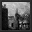
\includegraphics[width=0.6\textwidth]{images/greyscale/alban-modified.png}
        \caption{Original Image}
    \end{figure}
    \begin{figure}[h]
        \centering
        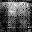
\includegraphics[width=0.6\textwidth]{images/outputs/noise/alban-modified_noise.png}
        \caption{Recovered Image}
    \end{figure}
    \begin{figure}[h]
        \centering
        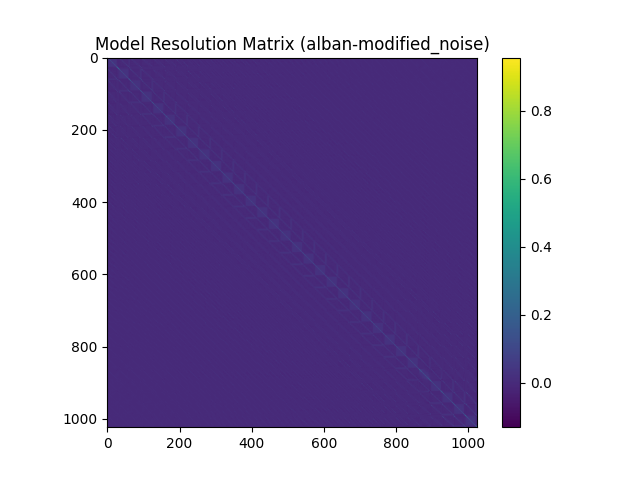
\includegraphics[width=1\textwidth]{images/outputs/modelres/alban-modified_noise.png}
        \caption{Model Resolution Matrix}
    \end{figure}
    \begin{figure}[h]
        \centering
        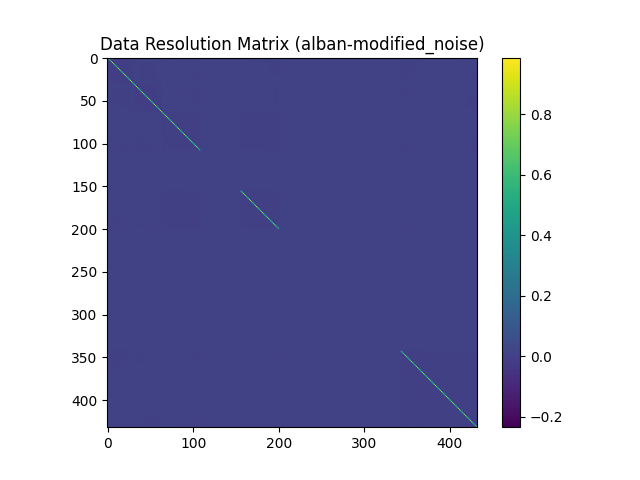
\includegraphics[width=1\textwidth]{images/outputs/datares/alban-modified_noise.png}
        \caption{Data Resolution Matrix}
    \end{figure}
    \clearpage


        \item aztec-modified\_noise
    \begin{figure}[h]
        \centering
        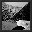
\includegraphics[width=0.6\textwidth]{images/greyscale/aztec-modified.png}
        \caption{Original Image}
    \end{figure}
    \begin{figure}[h]
        \centering
        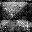
\includegraphics[width=0.6\textwidth]{images/outputs/noise/aztec-modified_noise.png}
        \caption{Recovered Image}
    \end{figure}
    \begin{figure}[h]
        \centering
        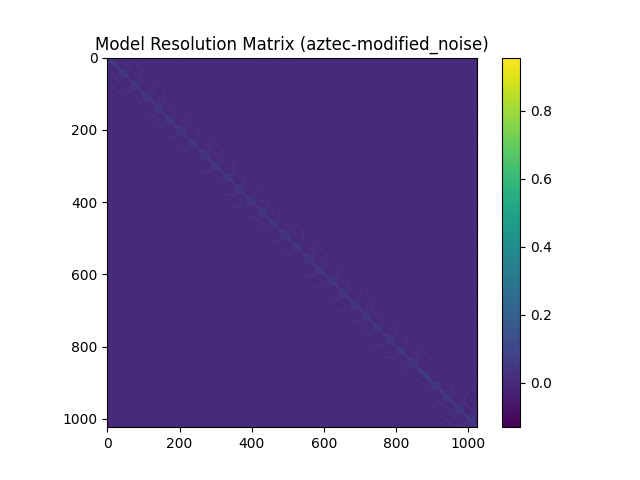
\includegraphics[width=1\textwidth]{images/outputs/modelres/aztec-modified_noise.png}
        \caption{Model Resolution Matrix}
    \end{figure}
    \begin{figure}[h]
        \centering
        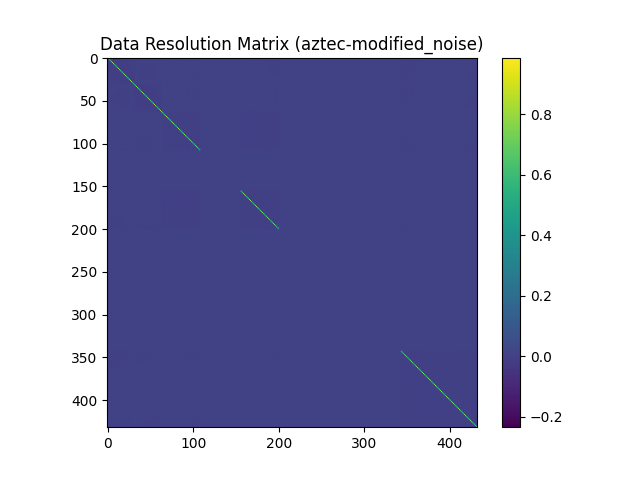
\includegraphics[width=1\textwidth]{images/outputs/datares/aztec-modified_noise.png}
        \caption{Data Resolution Matrix}
    \end{figure}
    \clearpage


        \item bee\_nest\_front\_honey-modified\_noise
    \begin{figure}[h]
        \centering
        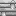
\includegraphics[width=0.6\textwidth]{images/greyscale/bee_nest_front_honey-modified.png}
        \caption{Original Image}
    \end{figure}
    \begin{figure}[h]
        \centering
        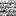
\includegraphics[width=0.6\textwidth]{images/outputs/noise/bee_nest_front_honey-modified_noise.png}
        \caption{Recovered Image}
    \end{figure}
    \begin{figure}[h]
        \centering
        \includegraphics[width=1\textwidth]{images/outputs/modelres/bee_nest_front_honey-modified_noise.png}
        \caption{Model Resolution Matrix}
    \end{figure}
    \begin{figure}[h]
        \centering
        \includegraphics[width=1\textwidth]{images/outputs/datares/bee_nest_front_honey-modified_noise.png}
        \caption{Data Resolution Matrix}
    \end{figure}
    \clearpage


        \item carved\_pumpkin-modified\_noise
    \begin{figure}[h]
        \centering
        \includegraphics[width=0.6\textwidth]{images/greyscale/carved_pumpkin-modified.png}
        \caption{Original Image}
    \end{figure}
    \begin{figure}[h]
        \centering
        \includegraphics[width=0.6\textwidth]{images/outputs/noise/carved_pumpkin-modified_noise.png}
        \caption{Recovered Image}
    \end{figure}
    \begin{figure}[h]
        \centering
        \includegraphics[width=1\textwidth]{images/outputs/modelres/carved_pumpkin-modified_noise.png}
        \caption{Model Resolution Matrix}
    \end{figure}
    \begin{figure}[h]
        \centering
        \includegraphics[width=1\textwidth]{images/outputs/datares/carved_pumpkin-modified_noise.png}
        \caption{Data Resolution Matrix}
    \end{figure}
    \clearpage


        \item cow\_noise
    \begin{figure}[h]
        \centering
        \includegraphics[width=0.6\textwidth]{images/greyscale/cow.png}
        \caption{Original Image}
    \end{figure}
    \begin{figure}[h]
        \centering
        \includegraphics[width=0.6\textwidth]{images/outputs/noise/cow_noise.png}
        \caption{Recovered Image}
    \end{figure}
    \begin{figure}[h]
        \centering
        \includegraphics[width=1\textwidth]{images/outputs/modelres/cow_noise.png}
        \caption{Model Resolution Matrix}
    \end{figure}
    \begin{figure}[h]
        \centering
        \includegraphics[width=1\textwidth]{images/outputs/datares/cow_noise.png}
        \caption{Data Resolution Matrix}
    \end{figure}
    \clearpage


        \item creeper\_noise
    \begin{figure}[h]
        \centering
        \includegraphics[width=0.6\textwidth]{images/greyscale/creeper.png}
        \caption{Original Image}
    \end{figure}
    \begin{figure}[h]
        \centering
        \includegraphics[width=0.6\textwidth]{images/outputs/noise/creeper_noise.png}
        \caption{Recovered Image}
    \end{figure}
    \begin{figure}[h]
        \centering
        \includegraphics[width=1\textwidth]{images/outputs/modelres/creeper_noise.png}
        \caption{Model Resolution Matrix}
    \end{figure}
    \begin{figure}[h]
        \centering
        \includegraphics[width=1\textwidth]{images/outputs/datares/creeper_noise.png}
        \caption{Data Resolution Matrix}
    \end{figure}
    \clearpage


        \item sheep\_noise
    \begin{figure}[h]
        \centering
        \includegraphics[width=0.6\textwidth]{images/greyscale/sheep.png}
        \caption{Original Image}
    \end{figure}
    \begin{figure}[h]
        \centering
        \includegraphics[width=0.6\textwidth]{images/outputs/noise/sheep_noise.png}
        \caption{Recovered Image}
    \end{figure}
    \begin{figure}[h]
        \centering
        \includegraphics[width=1\textwidth]{images/outputs/modelres/sheep_noise.png}
        \caption{Model Resolution Matrix}
    \end{figure}
    \begin{figure}[h]
        \centering
        \includegraphics[width=1\textwidth]{images/outputs/datares/sheep_noise.png}
        \caption{Data Resolution Matrix}
    \end{figure}
    \clearpage


        \item skeleton\_noise
    \begin{figure}[h]
        \centering
        \includegraphics[width=0.6\textwidth]{images/greyscale/skeleton.png}
        \caption{Original Image}
    \end{figure}
    \begin{figure}[h]
        \centering
        \includegraphics[width=0.6\textwidth]{images/outputs/noise/skeleton_noise.png}
        \caption{Recovered Image}
    \end{figure}
    \begin{figure}[h]
        \centering
        \includegraphics[width=1\textwidth]{images/outputs/modelres/skeleton_noise.png}
        \caption{Model Resolution Matrix}
    \end{figure}
    \begin{figure}[h]
        \centering
        \includegraphics[width=1\textwidth]{images/outputs/datares/skeleton_noise.png}
        \caption{Data Resolution Matrix}
    \end{figure}
    \clearpage


        \item steve\_noise
    \begin{figure}[h]
        \centering
        \includegraphics[width=0.6\textwidth]{images/greyscale/steve.png}
        \caption{Original Image}
    \end{figure}
    \begin{figure}[h]
        \centering
        \includegraphics[width=0.6\textwidth]{images/outputs/noise/steve_noise.png}
        \caption{Recovered Image}
    \end{figure}
    \begin{figure}[h]
        \centering
        \includegraphics[width=1\textwidth]{images/outputs/modelres/steve_noise.png}
        \caption{Model Resolution Matrix}
    \end{figure}
    \begin{figure}[h]
        \centering
        \includegraphics[width=1\textwidth]{images/outputs/datares/steve_noise.png}
        \caption{Data Resolution Matrix}
    \end{figure}
    \clearpage


        \item zombie\_noise
    \begin{figure}[h]
        \centering
        \includegraphics[width=0.6\textwidth]{images/greyscale/zombie.png}
        \caption{Original Image}
    \end{figure}
    \begin{figure}[h]
        \centering
        \includegraphics[width=0.6\textwidth]{images/outputs/noise/zombie_noise.png}
        \caption{Recovered Image}
    \end{figure}
    \begin{figure}[h]
        \centering
        \includegraphics[width=1\textwidth]{images/outputs/modelres/zombie_noise.png}
        \caption{Model Resolution Matrix}
    \end{figure}
    \begin{figure}[h]
        \centering
        \includegraphics[width=1\textwidth]{images/outputs/datares/zombie_noise.png}
        \caption{Data Resolution Matrix}
    \end{figure}
    \clearpage

\end{itemize}

\subsection{Observations:}
\begin{itemize}
    \item Smaller resolution images were recovered more accurately.
    \item Images that had more contrast were recovered mroe acurately.
    \item Images were clearer along the lines of rays used.
\end{itemize}

\section{Appendix Code:}

Make folder images\\
Make subfolders\\
images/greyscale\\
images/outputs\\ 
images/outputs/datares\\
images/outputs/modelres\\
images/outputs/noise\\
Place your greyscale images in images/greyscale, make sure not to use images with resolution higher than 64x64.
\subsection{main.py}
\begin{lstlisting}[style=python]
from matrix_tools import *
from img_tools import *
from grid import *
# note to self everything other than Line is generalisable to n dims in this code
def prod(lst):
    p = 1
    for a in lst:
        p *= a
    return p

def arr_indx_to_lst_indx(indx,arr_shape):
    lst_idx = 0
    for i in range(len(indx)):
        lst_idx += indx[i]*prod(arr_shape[:i])
    return lst_idx

def lst_indx_to_arr_indx(indx,arr_shape):
    arr_idx = []
    for i in range(len(arr_shape)-1,-1,-1):
        m = prod(arr_shape[:i])
        idx = indx//m
        indx = indx%m
        arr_idx.append(idx)
    arr_idx.reverse()
    return arr_idx

with_noise = True

img_names = ["alban-modified","aztec-modified","aztec2-modified","bee_nest_front_honey-modified","carved_pumpkin-modified","cow","creeper","fletching_table_front-modified","grass_block_side-modified","sheep","skeleton","steve","zombie"] 
for img_name in img_names:
    img = get_img(img_name+".png")
    arr = get_array(img)

    # img.show()
    img_shape = arr.shape
    print(img_shape)
    new_img = Image.fromarray(arr)
    # new_img.show()

    #making grid for passing light
    grid = Grid(1,dim=2)

    #passing light
    cells_information = []
    # light passing from below to up
    for x in range(img_shape[0]):
        source = (x+0.5,-1)
        ray = Line(91,source)
        cells = get_crossing_cells(grid,ray,((0,img_shape[0]),(0,img_shape[1])))
        cells_information.append(cells)
    #light passing from left to right
    for y in range(img_shape[1]):
        source = (-1,y+0.5)
        ray = Line(1,source)
        cells = get_crossing_cells(grid,ray,((0,img_shape[0]),(0,img_shape[1])))
        cells_information.append(cells)

    #light passing from diagonals
    line1 = Line(135,(-1,-1))
    num_sources = int(2*mt.ceil((img_shape[0]**2 + img_shape[1]**2)**(1/2)))
    sources = line1.get_points_distanced(0.5,num_sources)
    sources.extend(line1.get_points_distanced(-0.5,num_sources))
    for source in sources:
        ray = Line(45,source)
        cells = get_crossing_cells(grid,ray,((0,img_shape[0]),(0,img_shape[1])))
        cells_information.append(cells)

    line2 = Line(45,(img_shape[0]+1,img_shape[1]+1))
    sources = line2.get_points_distanced(0.5,num_sources)
    sources.extend(line2.get_points_distanced(-0.5,num_sources))
    for source in sources:
        ray = Line(135,source)
        cells = get_crossing_cells(grid,ray,((0,img_shape[0]),(0,img_shape[1])))
        cells_information.append(cells)





    #making F and d
    F = np.zeros((len(cells_information),prod(img_shape)))

    for i in range(len(cells_information)):
        # print(i)
        cells = cells_information[i] 
        for cell in cells:
            lst_idx = arr_indx_to_lst_indx(cell,img_shape)
            F[i,lst_idx] = 1


    m_real = np.reshape(arr,(prod(img_shape),1))

    d = np.matmul(F,m_real)
    if with_noise:
        img_name += "_noise"
        d = d + 0.05*d*np.random.normal(0,1,d.shape)

    print(F.shape)
    F_dag = tikonov_inverse(F)
    m_est = np.matmul(F_dag,d)
    model_res = np.matmul(F_dag,F)
    data_res = np.matmul(F,F_dag)
    matrix_img(model_res,"Model Resolution Matrix ("+img_name+")")
    plt.savefig("images/outputs/modelres/"+img_name)
    plt.show()
    matrix_img(data_res,"Data Resolution Matrix ("+img_name+")")
    plt.savefig("images/outputs/datares/"+img_name)
    plt.show()
    est_arr = np.reshape(m_est,img_shape)
    print(est_arr.shape)
    est_img = Image.fromarray(est_arr)
    est_img.show()
    est_img = est_img.convert('RGB')
    if with_noise:
        est_img.save("images/outputs/noise/"+img_name+".png")
    else:
        est_img.save("images/outputs/"+img_name+".png")

\end{lstlisting}

\subsection{grid.py}
\begin{lstlisting}[style=python]
    import math as mt
    # module for grid making and using the grid
    ''' 
    class makes a grid with cells numbered as (x,y,z) with no central cell
    The has centroid as coordinate point (0,0,0) is located at the intercetion of 8 cells 
    Grid extends infinitely on all sides 
    Cells are represented as a tuple of integers
    '''
    
    class Grid:
        def __init__(self,cell_dims,dim = 3):
            if not isinstance(cell_dims,tuple):
                self.is_cubic = True
                self.cell_size = cell_dims
                self.cell_dims = tuple([self.cell_size]*dim)
            else:
                self.is_cubic = False
                self.cell_dims = cell_dims
            self.dim = dim
        def get_cell(self, coords): #returns which cell the coords belong to
            if not isinstance(coords,tuple):
                raise Exception("Please enter a tuple")
            elif len(coords) != self.dim:
                raise Exception("Coordinate of ",self.dim,"dimensions expected")
            else:
                cell = []
                for i in range(self.dim):
                    x = coords[i] 
                    cell.append(int(x//self.cell_dims[i]))
            return tuple(cell)
        
        def get_cell_center(self,cell): #returns the center of the cell
            center_coords = []
            for i in range(self.dim):
                l = self.cell_dims[i]*cell[i]
                if l > 0:
                    coord = l - 0.5*self.cell_dims[i]
                else:
                    coord = l + 0.5*self.cell_dims[i]
                center_coords.append(coord)
            return tuple(center_coords)
    
    class Line:
        #creates a line passing through a point and having angle theta with +X axis (counter clockwise in degrees)
        def __init__(self,theta,point):
            self.theta = theta
            self.point = point
            self.m = mt.tan(mt.radians(theta))
            self.c = point[1]-self.m*point[0]
        
        def y(self,x): 
            return self.m*x+self.c
        
        def x(self,y):
            return (y-self.c)/self.m
        
        def get_point(self,d): #point at distance d from source
            x0, y0 = self.point[0], self.point[1]
            cstheta = mt.cos(mt.radians(self.theta))
            sntheta = mt.sin(mt.radians(self.theta))
            x, y = x0 + d*cstheta, y0 + d*sntheta
            return x,y
        
        def get_points_distanced(self,s,n): #n points equally distanced (s) from source 
            points = []
            for i in range(n):
                d = (i+1)*s
                points.append(self.get_point(d))
            return points
        
        def get_points_distanced_starting(self,start_dist,s,n):
            points = []
            for i  in range(n):
                d = start_dist + (i+1)*s
                points.append(self.get_point(d))
            return points
    
    def dist(x,y):
        S = 0 
        for i,j in zip(x,y):
            S += (i-j)**2
        S **= 1/2
        return S
    
    def get_crossing_cells(grid:Grid,line:Line,rang=((0,1000),(0,1000))): #get all the cells that the line crosses in a given range
        #0 included and 1000 not included
        sizes = []
        for pair in rang:
            sizes.append(pair[1]-pair[0])
        num_points_to_check = 0
        for s in sizes:
            num_points_to_check += s**2
        num_points_to_check **= 1/2
        num_points_to_check = int(mt.ceil(num_points_to_check))
        num_points_to_check *= 2
        points = []
        source = line.point
        pos_point1 = (rang[0][0],line.y(rang[0][0]))
        pos_point2 = (rang[0][1],line.y(rang[0][1]))
        pos_point3 = (line.x(rang[1][0]),rang[1][0])
        pos_point4 = (line.x(rang[1][1]),rang[1][1])
        pos_points = [pos_point1,pos_point2,pos_point3,pos_point4]
        to_remove = []
        for pos_point in pos_points:
            if pos_point[0] < rang[0][0] or pos_point[0] > rang[0][1] or pos_point[1] < rang[1][0] or pos_point[1] > rang[1][1]:
                to_remove.append(pos_point)
        for del_point in to_remove:
            pos_points.remove(del_point)
        if pos_points != []:
            pos_points.sort(key= lambda x: dist(source,x))
            closest_pt = pos_points[0]
            # print(closest_pt)
            start_dist = dist(source,closest_pt) - 0.5
            # print(start_dist)
            points.extend(line.get_points_distanced_starting(start_dist,0.5,num_points_to_check))
            points.extend(line.get_points_distanced_starting(start_dist,-0.5,num_points_to_check))
            points.extend(line.get_points_distanced_starting(-start_dist,-0.5,num_points_to_check))
            points.extend(line.get_points_distanced_starting(-start_dist,0.5,num_points_to_check))
        else:
            points = []
        cells = []
        for point in points:
            cell = grid.get_cell(point)
            if cell in cells:
                continue
            for i in range(len(cell)):
                c = cell[i]
                lr = rang[i][0]
                ur = rang[i][1]
                if c < lr or c >= ur:
                    break
            else:
                cells.append(cell)
        
        return cells
    
    # line = Line(90,(5.5,15))
    
    # grid = Grid(1,dim=2)
    # cells = get_crossing_cells(grid,line,((0,10),(0,10)))
    # print(cells)
    
\end{lstlisting}

\subsection{img\_tools.py}
\begin{lstlisting}[style=python]
from PIL import Image
import numpy as np

def get_img(img_name):
    img = Image.open("images/greyscale/"+img_name)
    return img

def get_array(img):
    arr = np.array(img)[:,:,0]
    return arr

\end{lstlisting}

\subsection{matrix\_tools.py}
\begin{lstlisting}[style=python]
import numpy as np
import matplotlib.pyplot as plt
np.random.seed(0)

def tikonov_inverse(F:np.ndarray,k = 0.1):
    return np.matmul(np.linalg.inv((np.matmul(F.transpose(),F)+k*np.identity(F.shape[1]))),F.transpose())

def tikonov_est(F:np.ndarray,d:np.ndarray,k = 0.1):
    return np.matmul(tikonov_inverse(F,k),d)

def generate_random_model(deg:int,rng:tuple):
    '''
    Enter a degree and a range and a model is generated for that range and degree
    '''
    m = np.random.uniform(low = rng[0], high = rng[1], size = (deg+1,1))
    return m

def gen_random_data(model:np.ndarray,size = 20, noise = 0.1,rng = (-10,10)):
    '''
    Enter a model, and data is generated for that model with added guassian noise
    '''
    f_0 = np.random.uniform(low = rng[0], high = rng[1], size = (size,1))
    F = np.concatenate([f_0**i for i in range(len(model))], axis=1)
    d_true = np.matmul(F,model) 
    d = d_true + noise*d_true*np.random.normal(0,1,d_true.shape)
    return F,d

def plot_model(m:np.ndarray,label:str,color:str):
    P = list(m.transpose()[0])
    P.reverse()
    poly_obj = np.poly1d(P)
    X = np.linspace(-10,10,100)
    plt.plot(X,poly_obj(X),label = label,c = color)   

def matrix_img(M:np.ndarray,title:str):
    plt.imshow(M)
    plt.title(title)
    plt.colorbar()


# m = generate_random_model(6,(-1,1))
# F,d = gen_random_data(m,size =3 ,noise=0)
# m_est = tikonov_est(F,d,k=1)
# plot_model(m,"True",'g')
# # plot_model(m_est,"Est",'r')
# plt.show()
\end{lstlisting}

\end{document}